\documentclass[10pt]{article}
\usepackage{icmlko}

\icmlmeta{IP 파운데이션 월드모델}{219}{여든여섯 노트 동안 실려 있던 갈래}{매 사이클 프롬프트 맨 아래에 적혀 있던 문턱 40→15 를 드디어 쟀다. 값이 없다 --- 그리고 그것을 연 근거가 부호까지 뒤집혔다}

\begin{document}

\twocolumn[
\icmlheader

\begin{abstract}
노트 133이 ``학습 문턱 40 은 노트 5의 편의값이고, 15 로 낮추면 짝 순위
우도가 팝업에서 $+$0.3698 에서 $+$0.4300 으로 오른다''를 적었다. 그 뒤로
\textbf{여든여섯 노트 동안} 그 한 줄이 매 사이클 프롬프트의 열린 갈래
목록에 실려 다녔다. 쟀다. \textbf{값이 없다.} 판이 F6 $+$0.4288 $\to$
$+$0.4293($t{=}1.33$) · F21 $+$0.4395 $\to$ $+$0.4395($t{=}-0.12$) ·
F18 $+$0.4396 $\to$ $+$0.4398($t{=}0.13$) · F9 $+$0.4280 $\to$
$+$0.4293($t{=}0.97$)로 \textbf{넷 다 유의하지 않다.} 문턱이 무엇을
가르는지부터 확인했다 --- \textbf{팝업 하나다.} T 이전 건수가 팝업 16 건
이고 나머지 아홉은 54$\sim$2,648 건이라, 40 이든 15 든 팝업이 학습 풀에
들어가느냐만 바뀐다(프롬프트에 적혀 있던 그대로다). 그럼 팝업에서는
어떤가. \textbf{부호가 갈린다} --- F6 $+$0.0074 · F21 $+$0.0047 인데
F18 $-$0.0002 · \textbf{F9 $-$0.0087} 이다. \textbf{노트 133 을 연 바로
그 정식화가 이제 반대로 움직인다.} 갈라 보면 양쪽이 다 움직였다 --- F9 의
팝업이 문턱 40 에서 $+$0.3698 이었는데 지금은 $+$0.3875 이고(기준선이
올랐다), 문턱 15 에서 $+$0.4300 이었는데 지금은 $+$0.3789 다(처치가
내렸다). \textbf{그 사이 팝업 빌드가 바뀌고}(노트 127의 넓은 판)
\textbf{축 무리가 셋 늘었으며}(검색 · 달력 · 위키) \textbf{자료 고침이 넷
있었다}(노트 207 · 210 · 213 · 214). \textbf{팝업이 다른 데서 좋아지자
그 16 건의 한계 가치가 사라졌다} --- 노트 217의 포화가 도메인 안에서도
같은 모양으로 나타난다. 문턱은 40 으로 둔다 --- 바꿀 근거가 점수뿐이고
그 점수도 유의하지 않다. \textbf{갈래를 닫는다.} 그리고 이 노트가 남기는
것은 문턱 값이 아니라 절차다: \textbf{열린 갈래 목록은 삭는다.} 여든여섯
노트 전에 잰 근거로 오늘의 우선순위를 정하고 있었다.
\end{abstract}
]

\begin{figure*}[t]
\centering
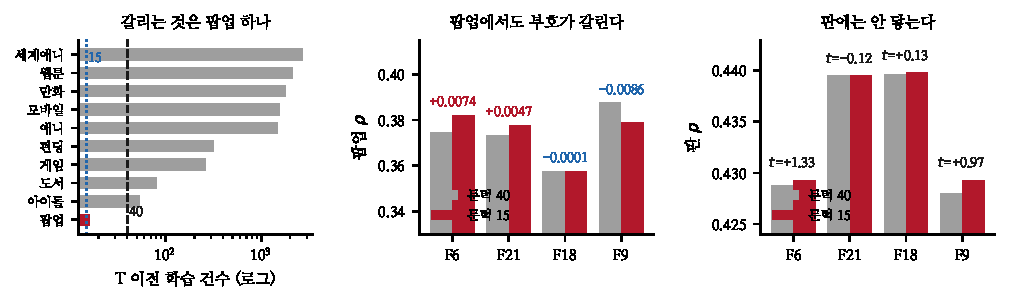
\includegraphics[width=\textwidth]{figs/threshold.pdf}
\caption{왼쪽 --- 갈리는 것은 팝업 하나. 가운데 --- 팝업에서도 부호가
갈린다. 오른쪽 --- 판에는 안 닿는다.}
\end{figure*}

\section{갈리는 것은 팝업 하나}

\begin{table}[t]
\centering\tsize
\caption{T(2025) 이전 학습 건수.}
\begin{tabular}{lrcc}
\toprule
& 건수 & 문턱 40 & 문턱 15 \\
\midrule
\textbf{팝업} & \textbf{16} & \textbf{×} & \textbf{○} \\
아이돌 & 54 & ○ & ○ \\
도서 & 80 & ○ & ○ \\
게임 & 259 & ○ & ○ \\
펀딩 & 320 & ○ & ○ \\
애니 & 1{,}467 & ○ & ○ \\
웹툰 & 2{,}106 & ○ & ○ \\
세계애니 & 2{,}648 & ○ & ○ \\
\bottomrule
\end{tabular}
\end{table}

\claimx{\textbf{문턱은 팝업 하나만 가른다.} 다음으로 작은 아이돌이 54 건
이라 40 과 15 사이에 아무도 없다.}{프롬프트에 그렇게 적혀 있었고 사실이다.
\textbf{그러면 이 갈래는 ``팝업 16 건을 학습 풀에 넣을 것인가'' 한 물음이다.}}

\section{팝업에서도 부호가 갈린다}

\begin{table}[t]
\centering\tsize
\caption{팝업 유보 $\rho$(59 건).}
\begin{tabular}{lrrr}
\toprule
& 문턱 40 & 문턱 15 & 차 \\
\midrule
F6 능형 & .3745 & .3819 & $+$.0074 \\
F21 & .3730 & .3777 & $+$.0047 \\
F18 배깅 & .3576 & .3575 & $-$.0002 \\
\textbf{F9 순위우도} & \textbf{.3875} & \textbf{.3789} & \textbf{$-$.0087} \\
\bottomrule
\end{tabular}
\end{table}

\claimx{\textbf{노트 133 을 연 바로 그 정식화가 반대로 움직인다.} 거기서는
F9 팝업이 $+$0.3698 $\to$ $+$0.4300 이었다 --- \textbf{$+$0.060 이 지금
$-$0.009 다.}}{양쪽이 다 움직였다 --- 기준선이 $+$0.3698 에서 $+$0.3875 로
오르고 처치가 $+$0.4300 에서 $+$0.3789 로 내렸다. \textbf{처치가 나빠진
것보다 기준선이 좋아진 몫이 크다.}}

\claimx{\textbf{팝업이 다른 데서 좋아지자 그 16 건의 한계 가치가
사라졌다.}}{그 사이 팝업 빌드가 넓어지고(노트 127) 축 무리가 셋 늘고
(검색 · 달력 · 위키) 자료 고침이 넷 있었다(노트 207 · 210 · 213 · 214).
\textbf{노트 217의 포화가 도메인 \emph{안에서도} 같은 모양이다} ---
바탕이 좋아지면 옛 지렛대의 값이 준다.}

\section{판에는 안 닿는다}

\begin{table}[t]
\centering\tsize
\caption{판 $\rho$. 짝 붓스트랩 500 회.}
\begin{tabular}{lrrr}
\toprule
& 문턱 40 & 문턱 15 & $t$ \\
\midrule
F6 능형 & .4288 & .4293 & 1.33 \\
F21 & .4395 & .4395 & $-$0.12 \\
F18 배깅 & .4396 & .4398 & 0.13 \\
F9 순위우도 & .4280 & .4293 & 0.97 \\
\bottomrule
\end{tabular}
\end{table}

\claimx{\textbf{넷 다 유의하지 않다.} 팝업이 판의 2.3\% 라 팝업 $\rho$ 가
$+$0.0074 올라도 판은 $+$0.0002 다.}{\textbf{문턱은 40 으로 둔다} ---
바꿀 근거가 점수뿐이고 그 점수도 유의하지 않다. 노트 210의 규칙대로
점수가 아니라 측정의 유효성으로 정해야 하는데, \textbf{여기서는 유효성이
양쪽 다 성립한다}(16 건으로 세운 계수도 정의는 된다).}

\section{갈래 목록이 삭는다}

\claimx{\textbf{이 노트가 남기는 것은 문턱 값이 아니라 절차다.}
여든여섯 노트 전에 잰 근거($+$0.060)로 오늘의 우선순위를 정하고
있었다.}{그 사이 판이 네 번 고쳐지고 축이 셋 늘고 챔피언이 두 번 바뀌었다.
\textbf{열린 갈래는 자료가 아니라 그때의 측정이고, 측정은 판이 바뀌면
삭는다.}}

\claimx{\textbf{같은 검사를 남은 갈래에도 해야 한다.} 지금 목록에 남은
것은 ``모바일 · 게임 검색 덮음 30$\sim$41\%''와 ``과제 78 시장 레코드
20 건 사람 태깅''이다.}{\textbf{후자는 이미 낡았다} --- 노트 154가
시장 레코드 51 건을 눈가림으로 읽어 매겼다. \textbf{목록이 그것을 모르고
있었다.}}

\begin{table}[t]
\centering\tsize
\caption{남은 것.}
\begin{tabular}{ll}
\toprule
\textbf{천장} & 무리마다 ``이 바탕 위 최대''를 표로 (측정 중) \\
\textbf{검색 덮음} & 남은 갈래 --- 천장부터 잴 것 \\
갈래 만료 & 갈래를 적을 때 잰 판 번호를 같이 적을 것 \\
\bottomrule
\end{tabular}
\end{table}

첫 줄이 이미 돌고 있고 이 노트를 일반화한다. 노트 218이 ``무리를 손보기
전에 그 무리의 천장을 먼저 계산하라''를 남겼고, 지금 무리 다섯을 각각
빼서 증분을 재고 있다. \textbf{첫 줄이 나왔는데 검색 무리의 천장이
$+$0.0365 다} --- 달력($+$0.015)의 두 배가 넘는다. \textbf{그러면 남은
갈래 ``검색 덮음 30$\sim$41\%''는 이 문턱 갈래와 달리 실제로 값이 있을
수 있고, 그 판단을 노트를 쓰기 \emph{전에} 할 수 있다.} 이것이 이 사이클이
얻은 절차다 --- 재기 전에 천장을 보고, 갈래를 적을 때 잰 시점을 같이 적는다.

\end{document}
